\DiaryEntry{Convolutional Codes, Viterbi Algorithm}{2019-03-25}{Coding}

Convolutional codes are linear codes that have additional structure in their generator matrix so that encoding can be interpreted as filtering (or convolution) operation. This allows easy implementation of an encoder.

\subsection{Code Structure, Encoder}

The encoder consists of $M$ 1-bit storage devices (shift registers) connected sequentially. The input information bits (denoted as $x_k$) pass from left to right through the shift registers. The outputs of the shift registers are xored together and form the $K$ different output streams. Which shift registers are xored together can be expressed by a binary vector; usually this vector is represented as octal number and called a generator polynom.

For example, assume two output streams ($K = 2$) denoted as $c_{k}^{(1)}$ and $c_{k}^{(2)}$, which we can express as follows

\begin{align*}
c_{k}^{(1)} &= x_k + x_{k-2} \\
c_{k}^{(2)} &= x_k + x_{k-1} + x_{k-2}
\end{align*}

This code would have generator polynomials $g_1 = 101_2 = 5_8$ and $g_2 = 111_2 = 7_8$ and require $M=2$ storage elements. A corresponding encoder is shown in the following Figure.

\begin{figure}[h]
  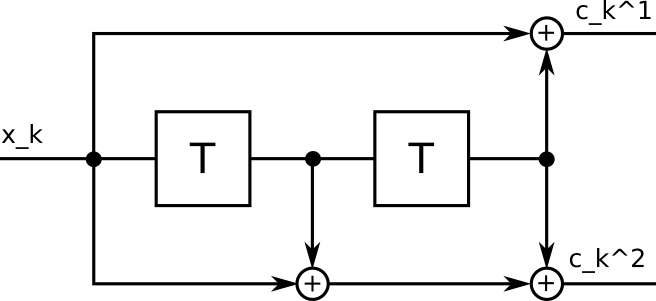
\includegraphics[scale=1.5]{images/convcodes_1_1.png}
\end{figure}


\subsection{Trellis Structure}

We can interpret the content of the $M$ shift registers as state (there are $2^M$ states) and the input values cause the values of the shift registers to change; i.e. state transitions. In addition, such a state transition produces an output (the $K$ values of $c_k^{(i)}$). The state transitions caused by inputs and the corresponding output can be visualized in a Trellis diagram. It shows the states (the content of the shift registers from left to right) before and after an input, with lines connecting the state transitions. A state transition is denoted by $b/c_1,\ldots c_k$.

The following Figure shows the Trellis diagram for the above code. For example, when in state $01$, an input $1$ causes a new state $10$ (the one from the input is shifted in from the left, causing the one on the right in the previous state to "falls out"), and an output of $00$.

\begin{figure}[h]
  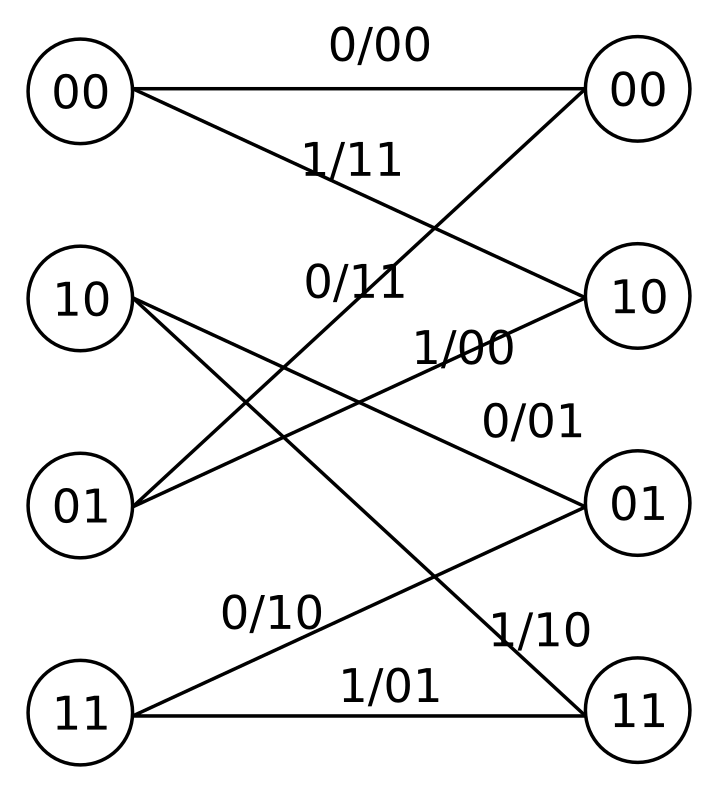
\includegraphics[scale=1.2]{images/convcodes_1_2.png}
\end{figure}



\subsection{Viterbi Decoding}

\subsubsection{Notation}

The input sequence $x_0, \ldots, x_{L-1}$ is denoted as vector $\xbf$. The vector of all $K$ codes bits at time $k$ is denoted as $\cbf_k$; the sequence of all code bits is denoted as $\cbf$. The code bits are mapped onto symbols $a$; for smplicity we assume a 1:1 mapping between code bits and symbols (e.g. BPSK). After the channel, the value $r$ is received.

We consider two channel models, a BSC channel with 

\bee
r = a \oplus n, \quad n \sim \Bc(p)
\eee

where $\Bc$ is a Bernoulli random variable with crossover probability $p$ and $\oplus$ denotes addition modulo-$2$.

Second channel model is an AWGN with

\bee
r = a + n, \quad n \sim \Nc(0, \sigma_w^2)
\eee

with $n$ distributed normally with zero-mean and variance $\sigma_{w}^2$.

For both channels $n$ is assumed to iid; resulting in a memoryless channel. The sequence of transmitted symbols is denoted as $\abf$ and the received values is denoted as $\rbf$.

We denote the likelihood of the channels with $f(r|a)$, in case of a BSC we have

\bee
f(r|a) = \left( \frac{p_c}{1-p_c}\right)^{d_H(r,a)} (1-p_c)^n
\eee

where $d_H$ denotes the Hamming distance between two binary values. For the AWGN we have


\bee
f(r|a) = \frac{1}{(\sqrt{2\pi \sigma_w^2)^n}} \exp \left\{ - \frac{1}{2\sigma_w^2} (r - a)^2 \right\}
\eee

\subsubsection{Algorithm Description}

We want to find the maximum likelihood sequence; i.e. the sequence $\xbf$ which maximizes $f(\rbf|\xbf)$. Since there is a one-to-one correspondence between $\xbf$, $\cbf$, and $\abf$, $f(\rbf|\xbf) = f(\rbf|\abf)$.

Maximizing the likelihood is equivalent to minimizing the metric; in case of the BSC the metric is $d_H(r,a)$; in case of the AWGN channel the metric is $(r-a)^2$.

The basic idea of the Viterbi algorithm is as follows. A sequence $\cbf$ (or, equivalently, $\abf$) corresponds to a path through the trellis. Due to channel noise, the received sequence may be different and the Viterbi decoder finds the sequence $\hat\cbf$ which is closest to the received $\rbf$ in terms of the metric (Hamming distance for the BSC, euclidean distance in case of the AWGN).

A naive approach would be to compute all paths through the trellis, calculate their metric (wrt to $\rbf$) and select the "closest" one. This is computationllay infeasible, as the number of paths grows exponentially with time.

The Viterbi algorithm is based on the observation that the path metric of a path can be expressed as sum of branch metrics. 

We introduce the following notation: The sequence $r_0,\ldots,r_{L-1}$ is denoted as $\rbf_{0}^{L-1}$ and the sequence $x_0,\ldots,x_{L-1}$ is denoted as $\xbf_{0}^{L-1}$. The likelihood is

\bee
f(\rbf|\xbf) = f(\rbf_{0}^{L-1} | \rbf_{0}^{L-1}) = \prod_{i=0}^{L-1} f(r_l|x_l)
\eee

which follows from the memoryless channel. Considering log-likelihoods instead, we have

\bee
\log f(\rbf|\xbf) = \log f(\rbf_{0}^{L-1} | \rbf_{0}^{L-1}) = \sum_{i=0}^{L-1} \log f(r_l|x_l)
\eee

Consider now a length-$N$ sequence $\xbf_{0}^{N-1}$ which leaves the trellis in state $\Psi_N = p$ at time $N$; the corresponding path through the trellis is denoted as $\Gamma_N = (\Psi_0,\ldots,\Psi_N)$. The log-likelihood of this sequence is

\bee
\log f(\rbf_{0}^{N-1} | \xbf_{0}^{N-1}) = \sum_{i=0}^{N-1} \log f(r_i|x_i)
\eee

and let $M_{N-1}(p) = -\log f(\rbf_{0}^{N-1} | \xbf_{0}^{N-1})$ denote the negative log-likelihood (or path metric) for this path $\Gamma_N$ which is defined by the sequence $\xbf_{0}^{N-1}$ and terminates in state $p$. 

Now let's see what happens when we append a symbol $\hat x_N$ to $\xbf_{0}^{N-1}$ and received value $r_N$ to $\rbf_{0}^{N-1}$. Suppose that the state at time $N+1$ is $\Psi_{N+1} = q$. The path metric for this longer path is then

\bee
M_N(q) = - \sum_{i=0}^{N} \log f(r_i|x_i) = - \sum_{i=0}^{N-1} \log f(r_i|x_i) - f(r_N|x_N) = M_{N-1}(p) - \log f(r_N|\hat x_N)
\eee

; i.e. it is the metric of the path $\Gamma_N$ (which is defined by the sequence $\xbf_{0}^{N-1}$ and terminates in state $p$) and a metric update moving the encoder from state $p$ to $q$.

The principle of the Viterbi algorithm is: To obtain the shortest path through the trellis, the path to state $q$ must be the shortest. When two paths merge into a state, the path with the smaller metric wins; i.e. it is retained and the other (longer) path is eliminated from futher consideration. The Viterbi algorithm keeps a list of paths into every state together with their metrics. When moving to the next state, it calculates all metric updates. Into state $p$, two paths merge from the previous time - the Viterbi algorithm adds the metric updates to the old metrics and finds the smallest of the two. It then updates the path into the new state together with the new metric.


This merging procedure is shown in the following Figure: Two previous states, $p_1, p_2$ merge into state $q$. The two previous states have path metrics $M_{N-1}(p_1)$ and $M_{N-1}(p_2)$, respectively. Transition from $p_1$ into $q$ is caused by $\hat x_1$ and transition from $p_2$ into $q$ is caused by $\hat x_2$. The observation of $r$ gives rise to the two likelihood values $f(r|\hat x_1)$ and $f(r|\hat x_2)$, respectively. This allows calculating two candidates for the path metric $M_N(q)$: One when the path from $p_1$ is used, one when the path from $p_2$ is used. With the arguments from above, the path with the smaller metric is selected while the other one is pruned.



\begin{figure}[h]
  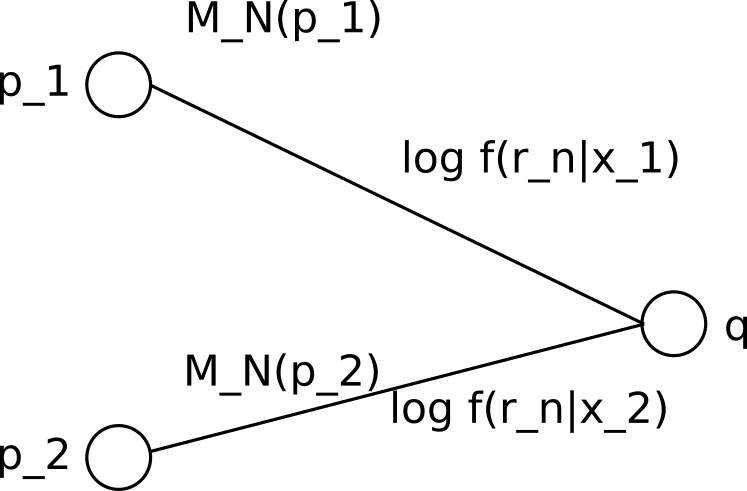
\includegraphics[scale=1.0]{images/convcodes_1_3.png}
\end{figure}


%%% Local Variables:
%%% mode: latex
%%% TeX-master: "journal"
%%% End:
